%%%%%%%%%%%%%%%%%%%%%%%%%%%%%%%%%%%%%%%%%
% Journal Article
% LaTeX Vzor
% Verzia 1.4 (15/5/16)
%
% Tento vzor bol stiahnutý z:
% http://www.LaTeXTemplates.com
%
% Pôvodný autor:
% Frits Wenneker (http://www.howtotex.com) s ďalšími upravami od
% Vel (vel@LaTeXTemplates.com)
%
% Licencia:
% CC BY-NC-SA 3.0 (http://creativecommons.org/licenses/by-nc-sa/3.0/)
%
%%%%%%%%%%%%%%%%%%%%%%%%%%%%%%%%%%%%%%%%%

%----------------------------------------------------------------------------------------
%	PACKAGES A ĎALŠIE UPRAVY DOKUMENTU
%----------------------------------------------------------------------------------------

\documentclass[twoside,twocolumn]{article}

\usepackage{blindtext} % Package to generate dummy text throughout this template 

\usepackage[sc]{mathpazo} % Palatino font
\usepackage[T1]{fontenc} % 8-bitove encodovanie ktore ma 256 glyphov
\linespread{1.07} % Line spacovanie - Palatino potrebuje viacej miesta medzi riadkami
\usepackage{microtype} 

\usepackage[english]{babel}

\usepackage[hmarginratio=1:1,top=32mm,columnsep=20pt]{geometry} % Rozsah dokumentu
\usepackage[hang, small,labelfont=bf,up,textfont=it,up]{caption} % 

\usepackage{booktabs} % Horizontalne pravidla pre tabulky

\usepackage{lettrine} % Prve velke pismeno na zaciatku textu 

\usepackage{enumitem} % Upravitelne lisy
\setlist[itemize]{noitemsep} % Make itemize lists more compact

\usepackage{abstract} % Allows abstract customization
\renewcommand{\abstracttextfont}{\normalfont\small\itshape} % Set the abstract itself to small italic text

\usepackage{titlesec} % Allows customization of titles
\renewcommand\thesection{\Roman{section}} % Roman numerals for the sections
\renewcommand\thesubsection{\roman{subsection}} % roman numerals for subsections
\titleformat{\section}[block]{\large\scshape\centering}{\thesection.}{1em}{} % Change the look of the section titles
\titleformat{\subsection}[block]{\large}{\thesubsection.}{1em}{} % Change the look of the section titles

\usepackage{fancyhdr} % Headers and footers
\pagestyle{fancy} % All pages have headers and footers
\fancyhead{} % Blank out the default header
\fancyfoot{} % Blank out the default footer
\fancyhead[C]{Toxicita a cheaty v FPS hrách $\bullet$ Nov 2022} % 
\fancyfoot[RO,LE]{\thepage} % Custom footer text

\usepackage{titling} % Customizing the title section
\usepackage{graphicx}
\usepackage{hyperref} % For hyperlinks in the PDF
\usepackage[export]{adjustbox}

%----------------------------------------------------------------------------------------
%	TITLE SEKCIA
%----------------------------------------------------------------------------------------

\setlength{\droptitle}{-4\baselineskip} % Posun titulku nahor

\pretitle{\begin{center}\Huge\bfseries} % Article titulok formatovanie zaciaotk
\posttitle{\end{center}} % Article titulok formatovanie koniec
\title{Toxicita a cheaty v FPS hrách} % Article titulok
\author{%
\textsc{Jakub Rafaj}\
\\[1ex]
\normalsize Fakulta informatiky a informačných technológií STU v Bratislave  \\%univerzita
\normalsize \href{mailto:rafaj.jakub@gmail.com}{rafaj.jakub@gmail.com} % emailova addresa
}
\date{\today} % datum
\renewcommand{\maketitlehookd}{%
}

%----------------------------------------------------------------------------------------

\begin{document}

% Vypisanie titulku
\maketitle

%----------------------------------------------------------------------------------------
%	ARTICLE OBSAH
%----------------------------------------------------------------------------------------

\section{Úvod}

\lettrine[nindent=0em,lines=3]{T}oxicita a cheaty\footnote[1]{Externy program, ktorý vám dáva kompetetívnu výhodu.} sú dve veľmi kontroverzné témy, ktoré by sa nemali len tak prehliadať. Preto by som sa v tomto článku chcel pozrieť na ich počiatky, ktoré zapríčinili ich výzor a výskyt v rôznych herných komunitách dnešnej doby. Komunitách populárnych hier ako sú napríklad: League of Legends od spoločnosti RIOT Games alebo Counter Strike Global Offensive od tvorcov VALVE.\\
Taktiež nazrieme na metódy a spôsoby, ako takéto spoločnosti bojujú proti rôznym druhom toxicity prostredníctvom samotných hráčov, ktorí pomocou report systému môžu poukázať na hráča, ktorý takto porušuje pravidlá, ktoré su uvedené v terms of service\footnote[2]{Pravidlá pri prevádzkovaní danej hry.} a ako bojujú proti cheatom\footnotemark[1], ktoré narušujú zábavu a zážitok, takto znevýhodnených hráčov. Ako prostriedky na boj proti cheatom\footnotemark[1] sú určené anti-cheaty\footnote[3]{Program, ktorý zisťuje výskyt cheatov.}, ktorých úlohou je sa zbavovať hráčov, ktorí takéto externe third party programy\footnote[4]{Program, ktorý pracuje mimo danej hry.} používajú vo svoj prospech, aby si vylepšili svoj herný výsledok, výkon a počet vyhraných hier, ktorý sa potom vykresľuje na ich výslednom ranku\footnote[5]{Ohodnotenie hráča podľa jeho herného výkonu.}.\\

%------------------------------------------------

\section{Metódy}

V tejto sekcii sú evedené metódy boja proti toxicite a cheatom\footnotemark[1].
\begin{itemize}
\item Terms of service\footnotemark[2] 
\item Report systém\footnote[6]{Nahlásovanie hráčov hráčmi.}
\item Anti-cheat\footnotemark[3]
\item Bannovanie\footnote[7]{Zakaz spustenia kompetetívnej hry na určitú dobu.}
\item Chat\footnote[8]{Prostredie na písanie pre hráčov} restrikcia
\end{itemize}
	Po inštalácii hry, hráči musia potvrdiť terms of service\footnotemark[2]t.j. kliknutí na tlačítko "Accept",čo značí potvrdenie.Terms of service\footnotemark[2] majú informovať hráča o rôznych priestupkoch, ktorých sa hráči nesmú dopustiť, ak nechcú byť potrestaný. Ak sa hráč dopustil priestupku a je zaznamenaný systémom, najčastejšie prostredníctvom anti-cheatu\footnotemark[3], alebo nahlásením tohto hráča iným hráčom.\\
	Report system\footnotemark[6] je jeden zo spôsobov, zachytavania priestupkov, ktorých sa hráči bežne dopúšťajú. Tieto priestupky sú nasledne ohlásené do systému hráčom, ktorý je vedomý priestupku, ktorého sa druhý hráč dopustil, alebo práve dopúšťa. Následne sú tieto sťažnosti od hráčov preverené ľuďmi na to určenými. Títo ludia overia pravdivosť sťažností a korektne potrestajú daného hráča, ktorý sa dopustil pristupku.\\
	Anti cheat\footnotemark[3] je program, ktorý je naprogramovaný na to, aby kontroloval hráčov a následne zistil výskyt third party programu\footnotemark[4], ktorý hráč používa, ako kompetetívnu výhodu a nasledne je korektne potrestaný.\\
	Banovanie\footnotemark[7] je spôsob trestania hráčov, ktorí sa dopustili priestupku, ktorý je v rozpore s terms of service\footnotemark[2]. Ak je hráč zabanovaný\footnotemark[7], tak je mu na určitý čas odoprená možnosť pripojiť sa do kompetetívnej hry.\\
	Chat\footnotemark[8] restrikcia je spôsob, akým hry zakazujú hráčom, ktorí porušili terms of service\footnotemark[2],na určitý čas písanie do chatu.

%------------------------------------------------

\section{Anti-cheat}
\subsection{Machine learning}
Machine Learning je jeden z typov anti-cheatov,ako je písané v \cite{willman2020machine}. Tento anti-cheat pracuje a vyhodnocuje svoje rozhodnutia na základe skúseností a rozhodnutí, ktoré vykonal v minulosti a na základe toho, či bolo to rozhodnuti správne , alebo chybné. Po dlhom čase budú rozhodnutia v značnej časti prevažne správne.\\
Machine learning funguje na podnetoch/vstupoch, ktoré získava z danej hry, nasledne tieto podnety/vstupy vyhodnocuje a podľa svojich skúseností vykoná akciu/výstup, ktorý je buď správny, alebo nesprávny.\\

\textnormal{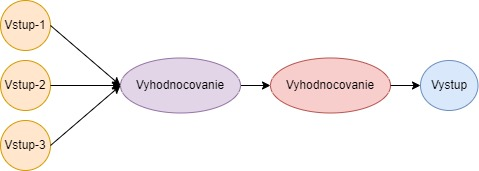
\includegraphics[scale=0.42]{Machine learning proces diagram.jpg}}
\label{machine learning proces}


\subsection{Subsection two}

%------------------------------------------------

\section{Discussion}

\subsection{Subsection One}

A statement requiring citation \cite{Figueredo:2009dg}.
\blindtext % Dummy text

\subsection{Subsection Two}

\blindtext % Dummy text

%----------------------------------------------------------------------------------------
%	REFERENCE LIST
%----------------------------------------------------------------------------------------
% Bibliographia
\bibliographystyle{elsarticle-num}
\bibliography{bibliography}


%----------------------------------------------------------------------------------------

\end{document}
